\documentclass{article}

%% preamble
\usepackage{hyperref}
\usepackage{verbatim}
\usepackage{color}
\usepackage{graphicx}
\usepackage{amsmath}

\topmargin 0pt
\advance \topmargin by -\headheight
\advance \topmargin by -\headsep
\textheight 9.in
\oddsidemargin 0pt
\evensidemargin \oddsidemargin
\marginparwidth 0.5in
\textwidth 6.5in
\newcommand{\myhrule}{ \begin{center}\rule{.9\linewidth}{.25mm}\end{center} }
\definecolor{darkgray}{rgb}{0.95,0.95,0.95}
\definecolor{heavygray}{rgb}{0.05,0.05,0.05}
\definecolor{foo}{rgb}{.8,0,.8}
\newcommand{\pad}{\vspace{8pt}\noindent}
\newcommand{\red}[1]{{\color{red}#1\color{black}}}
\newcommand{\myhref}[2]{\href{#1}{\color{foo}\underline{#2}\color{black}}}



\begin{document}

\title{CMDA 3634 Fall 2017 Homework 05}

%% change this to your name
\author{Kevin Jiang}
\vspace{-64pt}\maketitle
\begin{center}\underline{You must complete the following task by 11:59pm on 11/28/17.}\end{center}
Your write up for this homework should be presented in a {\LaTeX} formatted PDF document. You may copy the \LaTeX{} used to prepare this report as follows

\begin{enumerate}
\item Click on this  \myhref{https://www.sharelatex.com/project/5a0c6d0fe0f2720e611cca7f}{link} 
\item Click on Menu/Copy Project.
\item Modify the HW05.tex document to respond to the following questions. 
\item Remember: click the Recompile button to rebuild the document when you have made edits.
\item Remember: Change the author 
\item Instructions for assignment referred to in {\bf Q1} available on Canvas.
\end{enumerate}

\pad \emph{Each student} must individually upload the following files to the CMDA 3634 Canvas page at \myhref{https://canvas.vt.edu}{https://canvas.vt.edu}

\begin{enumerate}
\item \verb|firstnameLastnameHW05.tex| {\LaTeX} file.
\item Any figure files to be included by \verb|firstnameLastnameHW05.tex| file.
\item \verb|firstnameLastnameHW05.pdf| PDF file.
\item \verb|cudaMandelbrot.cu| and \verb|cudaJulia.cu| text file with student code. 
\end{enumerate}


\pad You must complete this assignment on your own. 

\vspace{16pt}
\begin{center}
\underline{\bf 90 points will be awarded for a successful completion.}
\vspace{8pt}\underline{\bf Extra credit will be awarded as appropriate.}
\end{center}

\newpage




\pad {\bf Q1} {\it (30 points) CUDA Mandelbrot.}
\vspace{8pt} 

\noindent 30 points will be awarded for completing the ``adding CUDA to a Mandelbrot set generator'' class assignment. Follow the instructions in the assignment PDF closely (available on Canvas). Remember to push the code to a HW5 sub directory in a repository that Dr. Warburton and William Winter have access to. Include the URL for the repository in your assignment write up.

\vspace{1em}


\noindent Copy and paste the contents of the batch script file used to submit a job to newriver into your \LaTeX{} report. Include the plot mentioned in (k) of the instructions in your report. Submit code to canvas (as well as pushing code to your GitHub repository).

\begin{verbatim}
#! /bin/bash

#PBS -l walltime=00:05:00
#PBS -l nodes=1:ppn=1:gpus=1
#PBS -W group_list=newriver
#PBS -q p100_dev_q
#PBS -A CMDA3634

cd $PBS_O_WORKDIR

module purge
module load cuda

nvcc -O3 -o mandelbrot -arch=sm_60 mandelbrot.cu png_util.c -I. -lpng -lm

./mandelbrot 4096 4096 32
./mandelbrot 4096 4096 64
./mandelbrot 4096 4096 128
./mandelbrot 4096 4096 256
./mandelbrot 4096 4096 512

rm mandelbrot

echo "Exited script normally"
\end{verbatim}

\begin{figure}[h!]
    \centering
    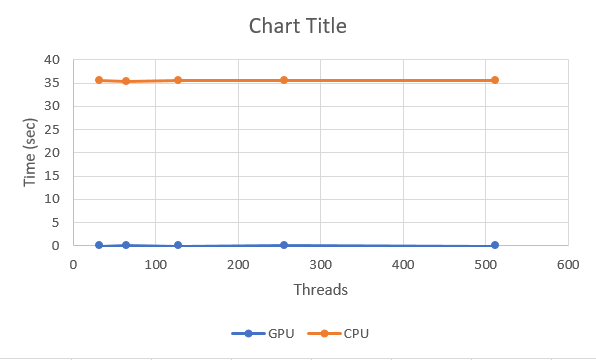
\includegraphics[scale=1]{gpu_cpu_mandelbrot.png}
    \caption{GPU vs CPU rendering times}
    \label{fig:gpu_cpu}
\end{figure}

\newpage
\myhrule

\pad {\bf Q2} {\it (30 points) CUDA Filled Julia Set.}
\vspace{8pt} 

\noindent Now we adapt the CUDA code from \textbf{Q1} to compute the Filled Julia Set for a particular value of $c$. When computing the Mandelbrot set, we fix an initial starting point $z = 0$ and vary $c$. To compute the Julia Set, we fix a particular $c$ and vary the starting point $z$. Copy the \verb|cudaMandelbrot.cu| code completed in \textbf{Q1} to a new file called \verb|cudaJulia.cu|. Edit the methods of the \verb|cudaJulia.cu| file according to the following instructions. 
\vspace{1em}

\noindent First edit the main function:
\begin{enumerate}
    \item Set \texttt{centRe} to $0$, \texttt{centIm} to $0$ and diam to $1.2$.
    \item Change \texttt{cmin}, \texttt{cmax}, and \texttt{dc} to \texttt{zmin}, \texttt{zmax}, and \texttt{dz} respectively. 
    \item Create a \texttt{complex\_t} type variable called $c$. Set $c$'s imaginary part to $0.1560$ and $c$'s real part to $-0.8$.
    \item Have the program call your \texttt{julia} kernel instead of \texttt{mandelbrot}. \texttt{julia} will have to take $c$ as an additional input. (See the instructions for the \texttt{julia} kernel below.)
    \item Change all instances of \texttt{mandelbrot} to \texttt{julia} in the remainder of the method.
\end{enumerate}
\vspace{1em}


\noindent Next change the \texttt{mandelbrot} kernel to a \texttt{julia} kernel:
\begin{enumerate}
    \item Choose the starting value for the complex variable $z$ based on the two-dimensional thread and block indices.  (Remember: We use a different $z$ value to initialize the iteration for each pixel of the final Julia image for a \emph{globally fixed} $c$.) 
    \item Add an additional \texttt{complex\_t} input that is the fixed $c$ used in the iteration. 
    \item Have threads call \texttt{testpoint}. (See below for changes to be made to \texttt{testpoint}.)
    \item Store the result of the \texttt{testpoint} method in the \texttt{julia} array. 
\end{enumerate}
\vspace{1em}


\noindent Lastly, update the \texttt{testpoint} method:
\begin{enumerate}
    \item Change the prototype so \texttt{testpoint} takes two \texttt{complex\_t} variables ($z$ and $c$).
    \item Since $z$ and $c$ are both inputs, delete the \texttt{complex\_t} $z$ declaration from the method.
\end{enumerate}
\vspace{1em}

\noindent Include the image generated by the program with the specified value of $c$ in your report ($c = -0.8 + 0.156 i$). Change values of $c$, \texttt{centRe}, \texttt{centIm}, and \texttt{diam} to produce different images. Extra credit will be awarded for cool Julia images. Submit code to canvas (as well as pushing code to your GitHub repository).

c value: -0.8 + 0.156i

\begin{figure}[h!]
    \centering
    
\includegraphics[scale=0.05]{julia_default.png}
    \caption{Changed Julia image set (diam=3.141592, centRe=-1.6, centIm=0.312)}
    \label{fig:default_julia}
\end{figure}

\begin{figure}[h!]
    \centering
    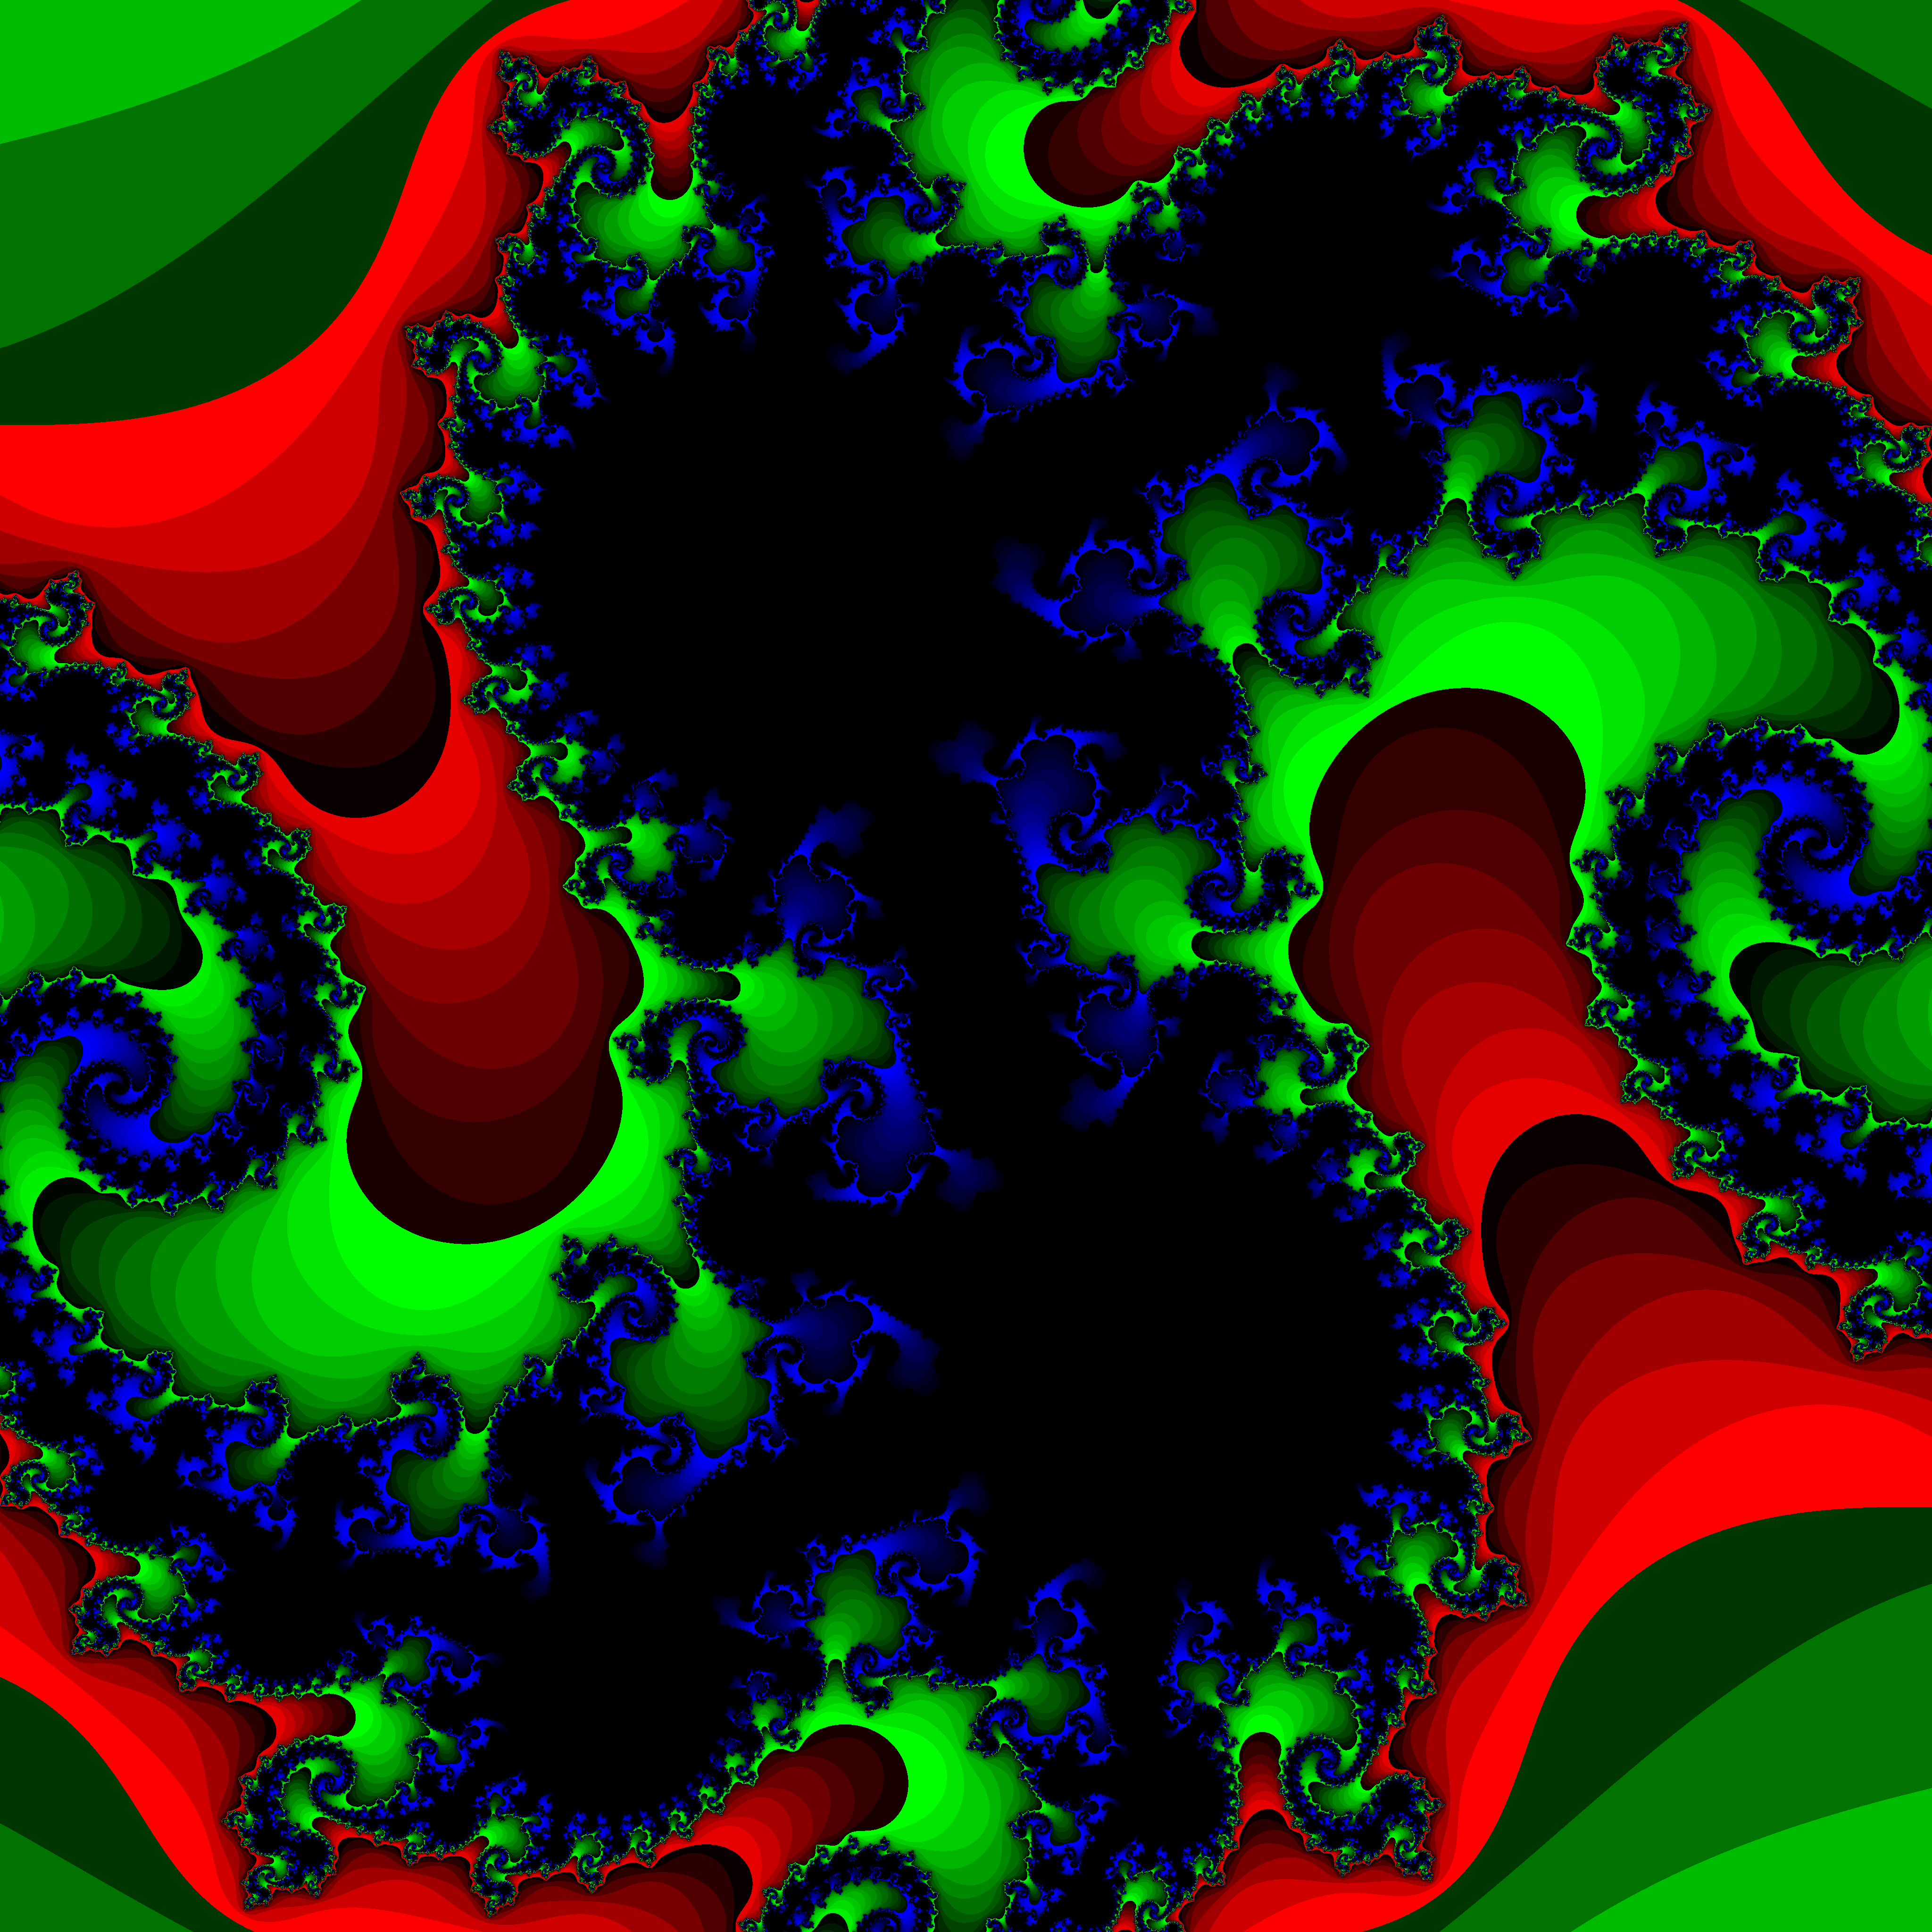
\includegraphics[scale=0.05]{julia.png}
    \caption{Original Julia image}
    \label{fig:julia}
\end{figure}

\newpage

\myhrule
\pad {\bf Q3} {\it (15 points) Profiling CUDA code.}
\vspace{8pt} 

\noindent Profile your CUDA Mandelbrot and CUDA Julia code from \textbf{Q1} and \textbf{Q2} using \texttt{nvprof}. Copy the output into your report. (Hint: Use \LaTeX{}'s verbatim environment.)

Mandelbrot output:
\begin{verbatim}
    elapsed = 0.010000
    Printing mandelbrot.png...done.
    elapsed = 0.020000
    Printing mandelbrot.png...done.
    elapsed = 0.010000
    Printing mandelbrot.png...done.
    elapsed = 0.020000
    Printing mandelbrot.png...done.
    elapsed = 0.010000
    Printing mandelbrot.png...done.
    Exited script normally
\end{verbatim}

Julia output:
\begin{verbatim}
    elapsed = 0.020000
    Printing julia.png...done.
\end{verbatim}

nvprof output:
\begin{verbatim}
    [kjiang@nr159 HW5]$ nvprof ./julia 4096 4096 32
    ==50577== NVPROF is profiling process 50577, command: ./julia 4096 4096 32
    elapsed = 0.020000
    Printing julia.png...done.
    ==50577== Profiling application: ./julia 4096 4096 32
    ==50577== Profiling result:
    Time(%)      Time     Calls       Avg       Min       Max  Name
    100.00%  21.454ms         1  21.454ms  21.454ms  21.454ms  [CUDA memcpy DtoH]
    
    ==50577== API calls:
    Time(%)      Time     Calls       Avg       Min       Max  Name
     92.26%  271.79ms         1  271.79ms  271.79ms  271.79ms  cudaMalloc
      7.51%  22.137ms         1  22.137ms  22.137ms  22.137ms  cudaMemcpy
      0.11%  316.94us         1  316.94us  316.94us  316.94us  cuDeviceTotalMem
      0.10%  299.87us        91  3.2950us     126ns  109.52us  cuDeviceGetAttribute
      0.01%  24.940us         1  24.940us  24.940us  24.940us  cuDeviceGetName
      0.00%  3.8410us         6     640ns     188ns  2.0320us  cudaSetupArgument
      0.00%  3.0740us         1  3.0740us  3.0740us  3.0740us  cudaLaunch
      0.00%  2.6820us         3     894ns     200ns  2.0730us  cuDeviceGetCount
      0.00%  1.3320us         1  1.3320us  1.3320us  1.3320us  cudaConfigureCall
      0.00%     898ns         3     299ns     190ns     475ns  cuDeviceGet
\end{verbatim}

\myhrule

\pad {\bf Q4} {\it (15 points) Memchecking CUDA code.}
\vspace{8pt} 

\noindent Run CUDA memcheck on your CUDA Mandelbrot and CUDA Julia code from \textbf{Q1} and \textbf{Q2} code. (For full credit, there should be no memory errors.) Copy the output into your report. (Hint: Use \LaTeX{}'s verbatim environment.) \\

After performing a cuda-memcheck on both files, I only come up with 1 error for a call to cudaLaunch.

Mandelbrot memory check:
\begin{verbatim}
    [kjiang@nr159 HW5]$ cuda-memcheck ./mandelbrot 4096 4096 32
    ========= CUDA-MEMCHECK
    ========= Program hit cudaErrorInvalidConfiguration (error 9) due to "invalid configuration argument" on CUDA API call to cudaLaunch. 
    =========     Saved host backtrace up to driver entry point at error
    =========     Host Frame:/lib64/libcuda.so.1 [0x2ef343]
    =========     Host Frame:./mandelbrot [0x376be]
    =========     Host Frame:./mandelbrot [0x36b7]
    =========     Host Frame:./mandelbrot [0x3306]
    =========     Host Frame:/lib64/libc.so.6 (__libc_start_main + 0xf5) [0x21b15]
    =========     Host Frame:./mandelbrot [0x343d]
    =========
    elapsed = 0.020000
    Printing mandelbrot.png...done.
    ========= ERROR SUMMARY: 1 error
\end{verbatim}

Julia memory check:
\begin{verbatim}
    [kjiang@nr159 HW5]$ cuda-memcheck ./julia 4096 4096 32
    ========= CUDA-MEMCHECK
    ========= Program hit cudaErrorInvalidConfiguration (error 9) due to "invalid configuration argument" on CUDA API call to cudaLaunch. 
    =========     Saved host backtrace up to driver entry point at error
    =========     Host Frame:/lib64/libcuda.so.1 [0x2ef343]
    =========     Host Frame:./julia [0x3771e]
    =========     Host Frame:./julia [0x3715]
    =========     Host Frame:./julia [0x331f]
    =========     Host Frame:/lib64/libc.so.6 (__libc_start_main + 0xf5) [0x21b15]
    =========     Host Frame:./julia [0x344d]
    =========
    elapsed = 0.020000
    Printing julia.png...done.
    ========= ERROR SUMMARY: 1 error
\end{verbatim}


%%\begin{thebibliography}{9}

%%\end{thebibliography}


\end{document}